\section{性能优化}
\label{sec:io_optimization}
下面介绍 \sys{} 的性能优化技术，重点在于降低 checkpoint 保存与加载相关开销。

\subsection{优化的 Plan 生成}
\label{sec:opt_plan}
\noindent \textbf{保存负载均衡}。
在采用 data parallelism（DP）的训练场景中，模型状态在所有 DP 组间复制，导致模型状态重复。
现有 checkpointing 系统~\cite{torch-dcp, megatron-dcp} 通常指定第一个 DP 组保存全部模型状态，但这会造成负载不均，使第一组成为 straggler。
为解决该问题，我们在规划阶段引入负载均衡的去重机制，采用 Worst-Fit 算法：协调者根据每个 tensor shard 的大小分配保存任务，总是将当前 shard 分配给累计 shard 大小最小的 rank。
这样可在各 rank 之间更均衡地分配保存负载，提升保存效率。
 
\noindent \textbf{消除冗余加载}。
当加载到包含 DP 的 parallelism 配置时，\sys{} 通过消除 DP 组间的重复读取来优化加载过程，将存储读取与 tensor 传输结合起来。
关键观察是：在文件读取期间，可利用空闲的跨 GPU 带宽同步把已加载 tensor 传给其他 GPU。
如图~\ref{fig:load_pipeline} 所示，在规划阶段我们将读取任务在 DP 组内均匀分配，避免重复读取；随后启动 I/O 线程读取分配的 tensor shards。
与此同时，在主线程中，CPU 内存中的 shards 先拷贝到 GPU，再通过 all-to-all 等集体通信传给需要的其他 worker。

\noindent \textbf{Plan 与 metadata 缓存}。
在大规模训练中，规划过程会带来显著的通信开销，尤其是在高频 checkpoint 保存时。
例如，为一个分布在 8960 GPUs 上的 405B transformer 模型规划保存流程需要 62 秒。
然而我们观察到，尽管 save plan 与全局 metadata 与具体 parallelism 绑定，但在同一次训练会话中保持不变。
因此可以通过缓存减少后续 checkpoint 操作的规划时间与开销。
我们引入 plan 与 metadata 缓存，将规划开销变为一次性成本。
首次生成后，save plan 与全局 metadata 可在后续复用，避免重复规划。

\subsection{全异步的 Engine Pipeline}
\label{sec:opt_pipeline}

\begin{figure}[!t]
  \centering
  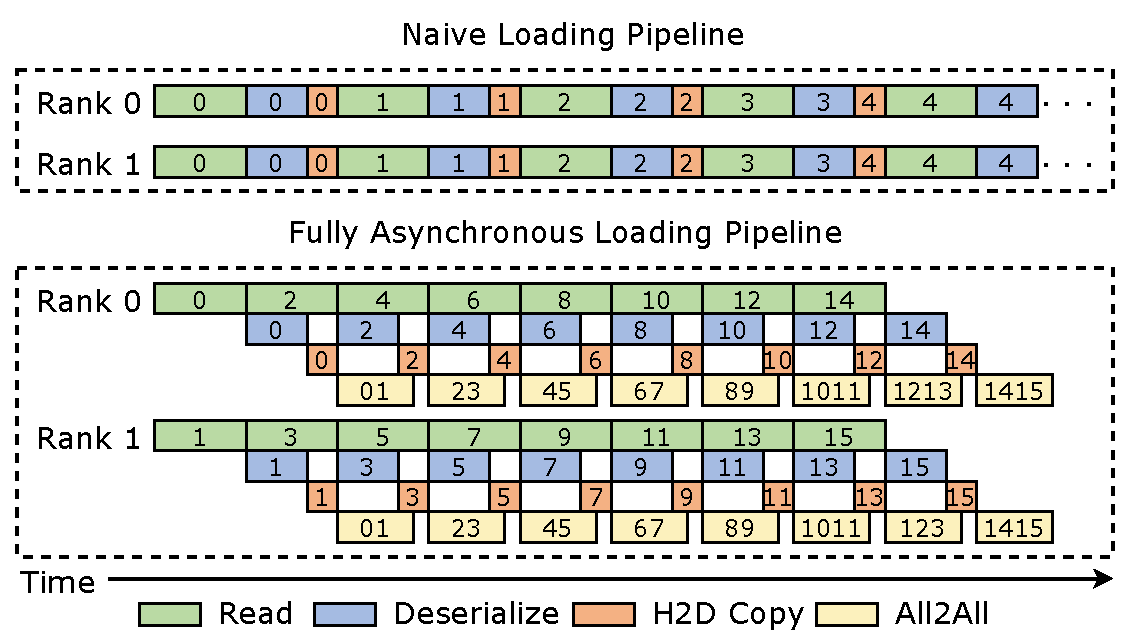
\includegraphics[width=\linewidth]{figures/load_pipeline.pdf}
  \caption{
   \sys{} 加载 pipeline 与朴素实现的对比。
  }
  \label{fig:load_pipeline}
\end{figure}

\sys{} 的 Engine 通过流水线化执行优化 checkpoint 保存与加载（resharding）。
以加载为例（图~\ref{fig:load_pipeline}），我们将每个 tensor shard 的文件读取、反序列化、Host-to-Device（H2D）拷贝以及 GPU 间通信进行流水线化，从而提升效率。
\textit{read} 操作会从存储系统下载包含所需 tensor 的文件，并放入共享内存（如 \texttt{dev/shm} 目录）；\textit{deserialize} 将共享内存中的内容反序列化为 tensor。
\sys{} 使用多线程并行进行文件下载与反序列化。
\textit{H2D copy} 将 tensor 从 CPU 内存传到 GPU，而 \textit{All2All} 在 DP 组内进行 tensor 传输。

对于保存，我们实现了对称的全异步 pipeline，包含 D2H 拷贝、序列化与文件上传。
为降低 D2H 对训练的影响，我们使用固定页（pinned）CPU 内存池，并结合 Ping-Pong 缓冲机制加速该操作。
此外，我们运行多个并行进程进行序列化并将文件写入共享内存。
上传线程在 dump 完成后自动检测并启动上传。

